\documentclass[a4paper,12pt]{article}
\usepackage[a4paper, margin=1in]{geometry} % Sets the paper size to A4 and margins to 1 inch
\usepackage{graphicx}
\usepackage{subcaption} % for subfigures
\usepackage{setspace}		
\usepackage{xcolor,listings} % for typesetting code
\usepackage{enumitem}
\usepackage{tabularx}

% Define SQL listing style
% \lstset{
%     language=SQL,
%     basicstyle=\ttfamily,
%     keywordstyle=\bfseries,
%     commentstyle=\itshape,
%     showstringspaces=false,
%     numbers=left,
%     numberstyle=\tiny,
%     numbersep=5pt,
%     breaklines=true,
%     frame=single,
%     backgroundcolor=\color{gray!10},
%     captionpos=b
% }
\lstset{
    upquote=true,
    language=SQL,
    showspaces=false,
    basicstyle=\ttfamily,
    keywordstyle=\bfseries\color{blue!60},
    numbers=left,
    numberstyle=\tiny,
    commentstyle=\color{gray},
    backgroundcolor=\color{gray!10}
}

\begin{document}


%% Adding logo
\begin{figure}[h]
		\vspace*{-1em}
		\centering
		
\includegraphics[width=0.2\linewidth]{university_logo.png}
		\par
		\vspace*{2em}
		{\Large UNIVERSITY OF CHITTAGONG}
\end{figure}
%% Document information
\begin{center}
		\vspace*{3em}
		\textbf{Department of Computer Science and Engineering} \\
		\bigskip
		Session: 2021-2022 \\
		4th semester \\
		\bigskip
		\begin{tabular}{l l}
		  Assignment No. &: 1\\
		  Course Title &: Database Systems \\
		  Course Code No. &: CSE-413 \\
		\end{tabular}
\end{center}

%% Teacher information
\begin{center}
		\vspace*{3em}
		Submitted to: \\
		\textbf{Dr. Rudra Pratap Deb Nath} \\
		Associate Professor \\
		Department of Computer Science and Engineering \\
		University of Chittagong
\end{center}

%% Student information
\begin{center}
		\vspace*{3em}
		Submitted by: \\
		\textbf{Sanzid Islam Mahi} \\
		ID: 22701065 \\
		Department of Computer Science and Engineering \\
		University of Chittagong
\end{center}




\begin{center}
	\vspace*{3em}
	Date: Jul 02, 2024
\end{center}

\newpage
\section*{Chapter 4}
\subsection*{Practice 4}
\begin{enumerate}
    \item Create a report that produces the following for each employee: \\
\textless employee last name\textgreater{} earns \textless salary\textgreater{} monthly but wants \textless 3 times
salary.\textgreater{}. Label the column Dream Salaries.

    \begin{figure}[h]
        \centering
            \centering
            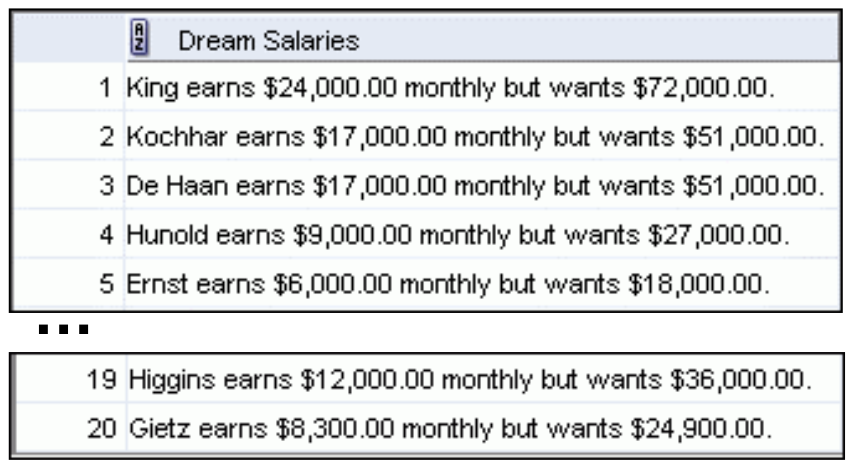
\includegraphics[width=.6\linewidth]{graphics/41.png}
    \end{figure}
    
    \textbf{Solution: }
    \begin{lstlisting}[language=SQL]
SELECT Last_Name || ' earns ' || Salary || 
    ' monthly but wants ' || (Salary * 3) || '.' 
    AS "Dream Salaries"
FROM hr.Employees;
    \end{lstlisting}
        \item Display each employee's last name, hire date, and salary review date, which is the first Monday
after six months of service. Label the column REVIEW. Format the dates to appear in the format
similar to “Monday, the Thirty-First of July, 2000.”

    \begin{figure}[h]
        \centering
            \centering
            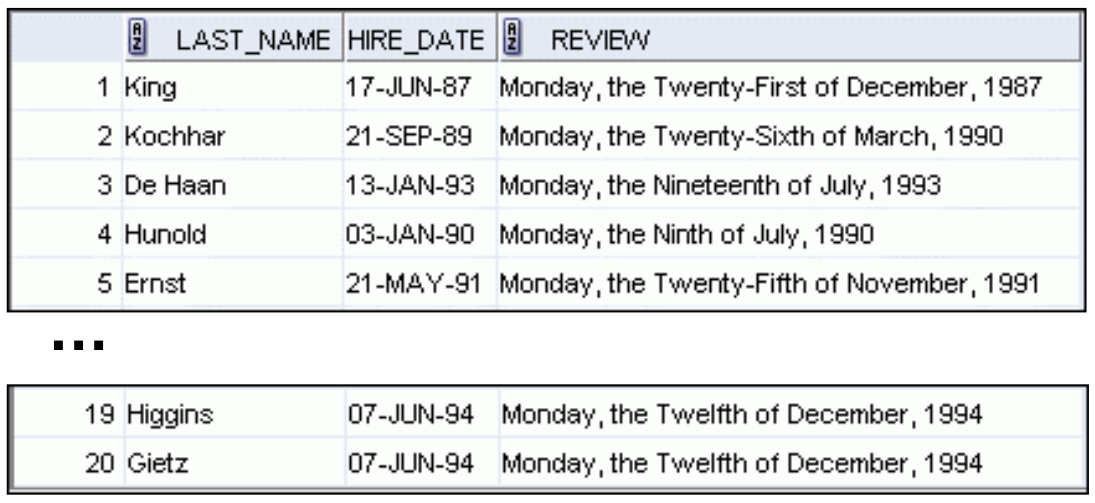
\includegraphics[width=.6\linewidth]{graphics/42.png}
    \end{figure}
    
    \textbf{Solution: }
    \begin{lstlisting}[language=SQL]
SELECT last_name, hire_date,
    TO_CHAR(
        NEXT_DAY(ADD_MONTHS(hire_date, 6) - 1, 'MONDAY'),
        'FMDay,"the" fmDdsp "of" FMMonth,YYYY'
    ) AS review
FROM hr.employees;
    \end{lstlisting}
    \newpage
    \item Display the last name, hire date, and day of the week on which the employee started. Label the
column DAY. Order the results by the day of the week, starting with Monday.
    \begin{figure}[h]
        \centering
            \centering
            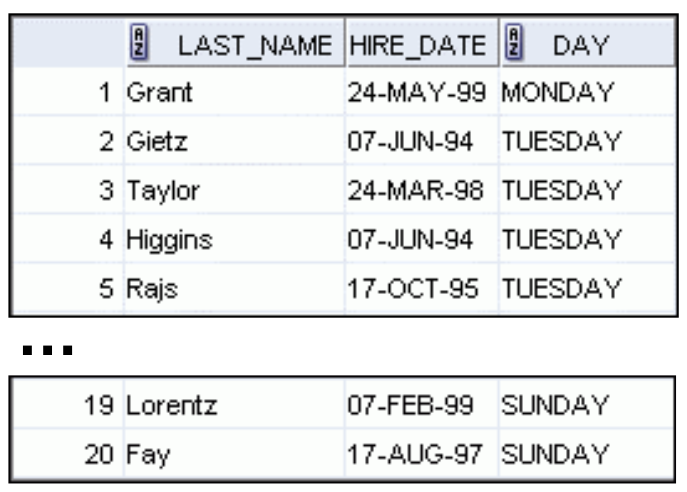
\includegraphics[width=.4\linewidth]{graphics/43.png}
    \end{figure}
    
    \textbf{Solution: }
    \begin{lstlisting}[language=SQL]
SELECT last_name,hire_date,
    TO_CHAR(hire_date, 'Day') AS DAY
FROM hr.employees
ORDER BY
    CASE
        WHEN TO_CHAR(hire_date, 'D') = '1' THEN 7
        ELSE TO_CHAR(hire_date, 'D') - 1
    END;
    \end{lstlisting}
        \item Create a query that displays the employees' last names and commission amounts. If an employee
does not earn commission, show “No Commission.” Label the column COMM.
    \begin{figure}[h]
        \centering
            \centering
            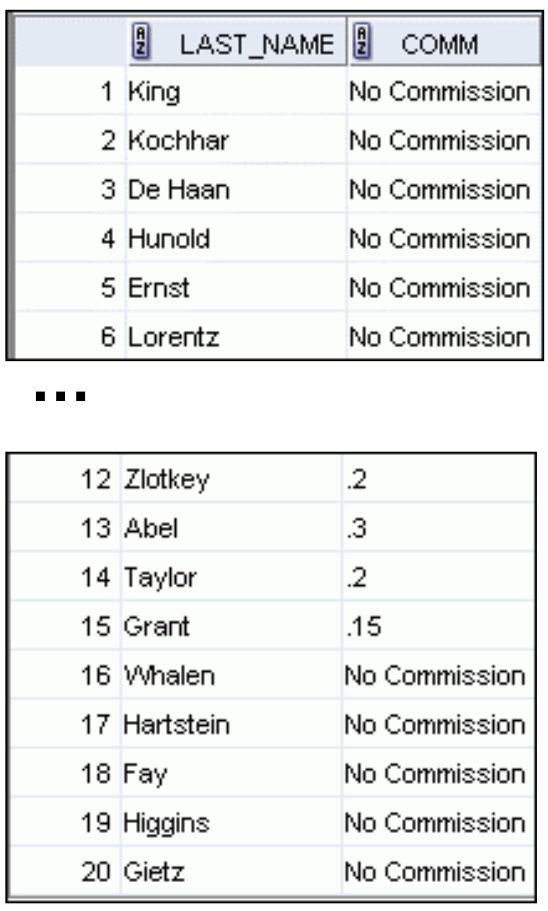
\includegraphics[width=.35\linewidth]{graphics/44.png}
    \end{figure}
    \newpage
    \textbf{Solution: }
    \begin{lstlisting}[language=SQL]
SELECT last_name,
    CASE 
        WHEN commission_pct IS NULL OR commission_pct = 0 
        THEN 'No Commission'
        ELSE TO_CHAR(commission_pct,'fm.99')
    END AS comm
FROM hr.employees;
    \end{lstlisting}
    % \newpage
        \item Using the DECODE function, write a query that displays the grade of all employees based on the
value of the column \texttt{JOB\_ID}, using the following data:
 
\begin{tabularx}{\textwidth}{lX}
\textbf{Job} & \textbf{Grade} \\
AD\_PRES & A \\
ST\_MAN & B \\
IT\_PROG & C \\
SA\_REP & D \\
ST\_CLERK & E \\
None of the above & 0 \\
\end{tabularx}
    
    \begin{figure}[h]
        \centering
            \centering
            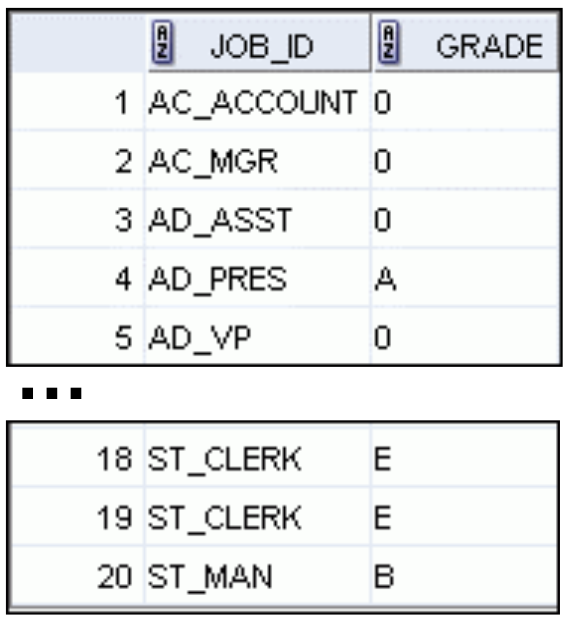
\includegraphics[width=.3\linewidth]{graphics/45.png}
    \end{figure}

    \textbf{Solution: }
    \begin{lstlisting}[language=SQL]
SELECT last_name,job_id,
    DECODE(job_id,
           'AD_PRES', 'A',
           'ST_MAN', 'B',
           'IT_PROG', 'C',
           'SA_REP', 'D',
           'ST_CLERK', 'E',
           '0'
    ) AS grade
FROM hr.employees;
    \end{lstlisting}
    \newpage
    \item Rewrite the statement in the preceding exercise using the CASE syntax.
    \begin{figure}[h]
        \centering
            \centering
            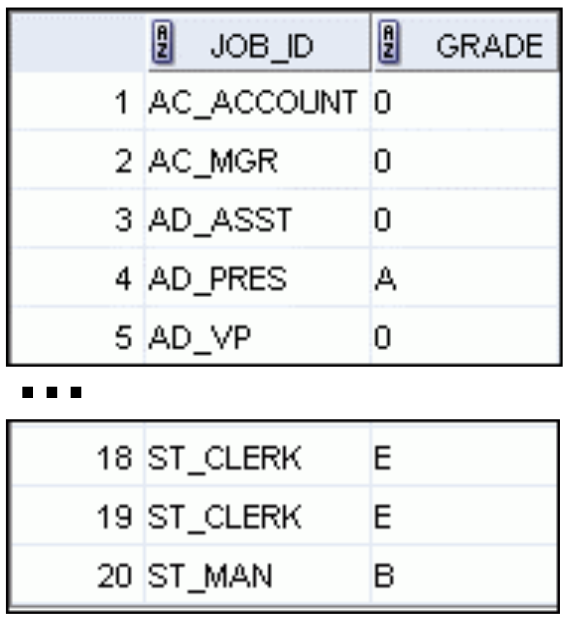
\includegraphics[width=.3\linewidth]{graphics/46.png}
    \end{figure}
    
    \textbf{Solution: }
    \begin{lstlisting}[language=SQL]
SELECT last_name,job_id,
    CASE job_id
        WHEN 'AD_PRES' THEN 'A'
        WHEN 'ST_MAN' THEN 'B'
        WHEN 'IT_PROG' THEN 'C'
        WHEN 'SA_REP' THEN 'D'
        WHEN 'ST_CLERK' THEN 'E'
        ELSE '0'
    END AS grade
FROM employees;

    \end{lstlisting}
\end{enumerate}

\newpage
\section*{Chapter 5}
\subsection*{practice 5}
\begin{enumerate}
    \item Group functions work across many rows to produce one result per group.\\
True/False\\\\
    \textbf{Answer: }\textcolor{blue}{True}
    \item Group functions include nulls in calculations. \\
True/False\\\\
    \textbf{Answer: }\textcolor{red}{False}
    \item The WHERE clause restricts rows before inclusion in a group calculation.\\
True/False\\\\
    \textbf{Answer: }\textcolor{blue}{True}

    \item     Find the highest, lowest, sum, and average salary of all employees. Label the columns
as Maximum, Minimum, Sum, and Average, respectively. Round your results to the nearest
whole number. Save your SQL statement as \texttt{lab\_05\_04.sql}. Run the query.
    \begin{figure}[h]
        \centering
        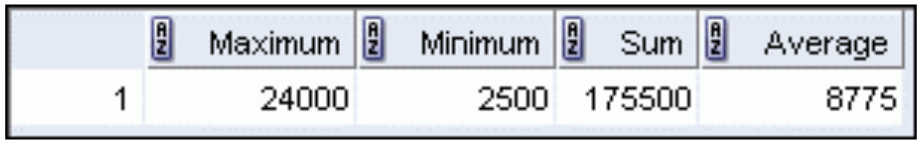
\includegraphics[width=.5\linewidth]{graphics/64.png}
    \end{figure}

    \textbf{Solution: }
    \begin{lstlisting}[language=SQL]
SELECT
    ROUND(MAX(salary)) AS "Maximum",
    ROUND(MIN(salary)) AS "Minimum",
    ROUND(SUM(salary)) AS "Sum",
    ROUND(AVG(salary)) AS "Average"
FROM hr.employees;
    \end{lstlisting}
    %problem 5
        \item Modify the query in \texttt{lab\_05\_04.sql} to display the minimum, maximum, sum, and average
salary for each job type. Resave \texttt{lab\_05\_04.sql} as \texttt{lab\_05\_05.sql}. Run the statement
in \texttt{lab\_05\_05.sql}.
    \begin{figure}[h]
        \centering
        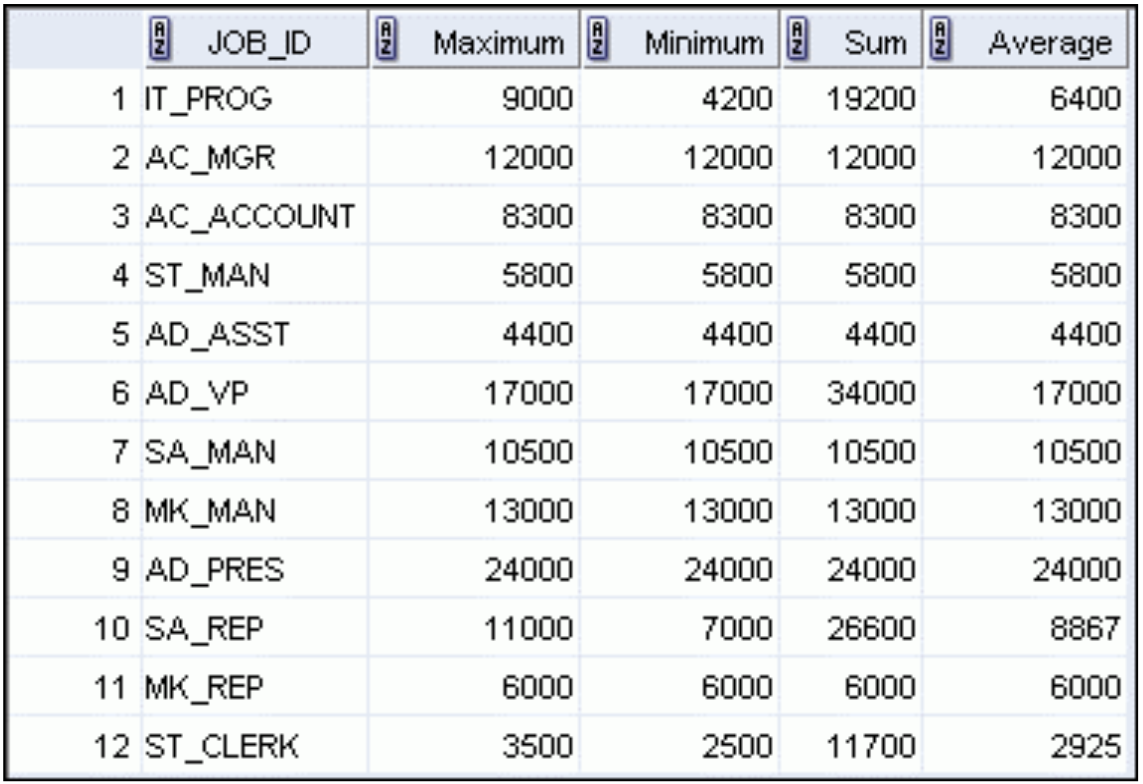
\includegraphics[width=.5\linewidth]{graphics/65.png}
    \end{figure}

    \textbf{Solution: }
    \begin{lstlisting}[language=SQL]
SELECT job_id,
    ROUND(MIN(salary)) AS "Minimum",
    ROUND(MAX(salary)) AS "Maximum",
    ROUND(SUM(salary)) AS "Sum",
    ROUND(AVG(salary)) AS "Average"
FROM hr.employees
GROUP BY job_id;
    \end{lstlisting}
    %problem 6
    \newpage
        \item Write a query to display the number of people with the same job.
    \begin{figure}[h]
        \centering
        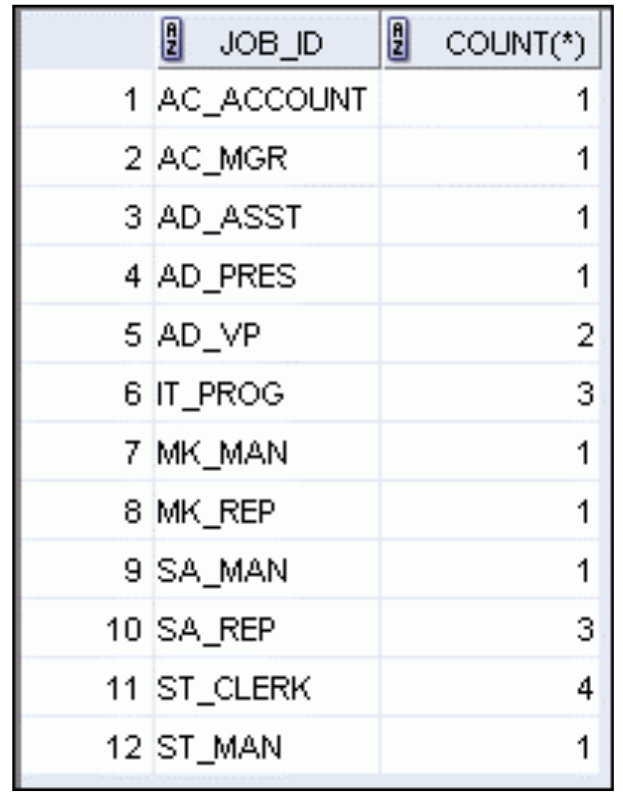
\includegraphics[width=.45\linewidth]{graphics/66.1.png}
    \end{figure}

    \textbf{Solution: }
    \begin{lstlisting}[language=SQL]
SELECT job_id, COUNT(*) 
FROM hr.employees
GROUP BY job_id;
    \end{lstlisting}
    Generalize the query so that the user in the HR department is prompted for a job title. Save the script
to a file named \texttt{lab\_05\_06.sql}. Run the query. Enter \texttt{IT\_PROG} when prompted.
    \begin{figure}[h]
        \centering
        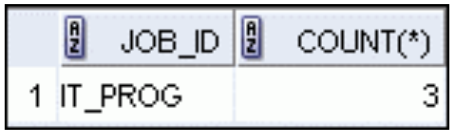
\includegraphics[width=.4\linewidth]{graphics/66.2.png}
    \end{figure}
%     \begin{lstlisting}[language=SQL]
% SELECT job_id , COUNT (*)
% FROM hr.employees
% WHERE job_id = upper ('&job_id')
% GROUP BY job_id ;
%     \end{lstlisting}

    \textbf{skipped}
    %problem 7
        \item Determine the number of managers without listing them. Label the column as Number of
Managers. Hint: Use the \texttt{MANAGER\_ID} column to determine the number of managers.
    \begin{figure}[h]
        \centering
        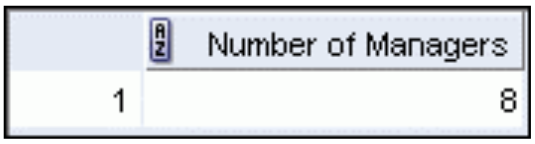
\includegraphics[width=.4\linewidth]{graphics/67.png}
    \end{figure}

    \textbf{Solution: }
    \begin{lstlisting}[language=SQL]
SELECT 
    COUNT(DISTINCT manager_id) AS "Number of Managers"
FROM hr.employees
WHERE manager_id IS NOT NULL;
    \end{lstlisting}
    %peoblem 8
    % \newpage
        \item Find the difference between the highest and lowest salaries. Label the column DIFFERENCE.
    \begin{figure}[h]
        \centering
        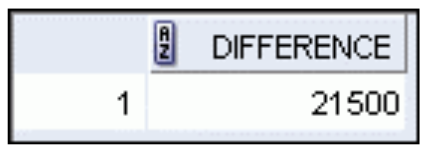
\includegraphics[width=.35\linewidth]{graphics/68.png}
    \end{figure}

    \textbf{Solution: }
    \begin{lstlisting}[language=SQL]
SELECT (MAX(salary) - MIN(salary)) AS DIFFERENCE
FROM hr.employees;
    \end{lstlisting}
        %peoblem 9
        \item Create a report to display the manager number and the salary of the lowest-paid employee for
that manager. Exclude anyone whose manager is not known. Exclude any groups where the
minimum salary is \$6,000 or less. Sort the output in descending order of salary.
    \begin{figure}[h]
        \centering
        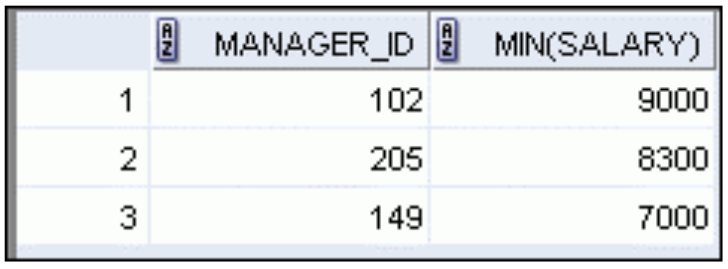
\includegraphics[width=.4\linewidth]{graphics/69.png}
    \end{figure}

    \textbf{Solution: }
    \begin{lstlisting}[language=SQL]
SELECT manager_id,MIN(SALARY)
FROM hr.employees
WHERE manager_id IS NOT NULL
GROUP BY manager_id
HAVING MIN(salary) > 6000
ORDER BY MIN(SALARY) DESC;
    \end{lstlisting}
    %peoblem 10
    \newpage
    \item Create a query to display the total number of employees and, of that total, the number of
employees hired in 1995, 1996, 1997, and 1998. Create appropriate column headings.
    \begin{figure}[h]
        \centering
        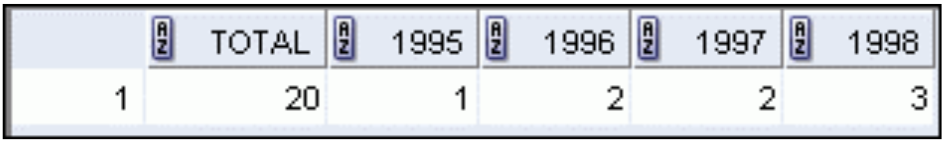
\includegraphics[width=.5\linewidth]{graphics/610.png}
    \end{figure}

    \textbf{Solution: }
    \begin{lstlisting}[language=SQL]
SELECT COUNT(*) AS "TOTAL",
    SUM(CASE WHEN TO_CHAR(hire_date, 'YYYY') = '1995' 
        THEN 1 ELSE 0 END) AS "1995",
    SUM(CASE WHEN TO_CHAR(hire_date, 'YYYY') = '1996' 
        THEN 1 ELSE 0 END) AS "1996",
    SUM(CASE WHEN TO_CHAR(hire_date, 'YYYY') = '1997' 
        THEN 1 ELSE 0 END) AS "1997",
    SUM(CASE WHEN TO_CHAR(hire_date, 'YYYY') = '1998'
        THEN 1 ELSE 0 END) AS "1998"
FROM hr.employees;
    \end{lstlisting}
    %peoblem 11
    \item Create a matrix query to display the job, the salary for that job based on department number,
and the total salary for that job, for departments 20, 50, 80, and 90, giving each column an
appropriate heading.
    \begin{figure}[h]
        \centering
        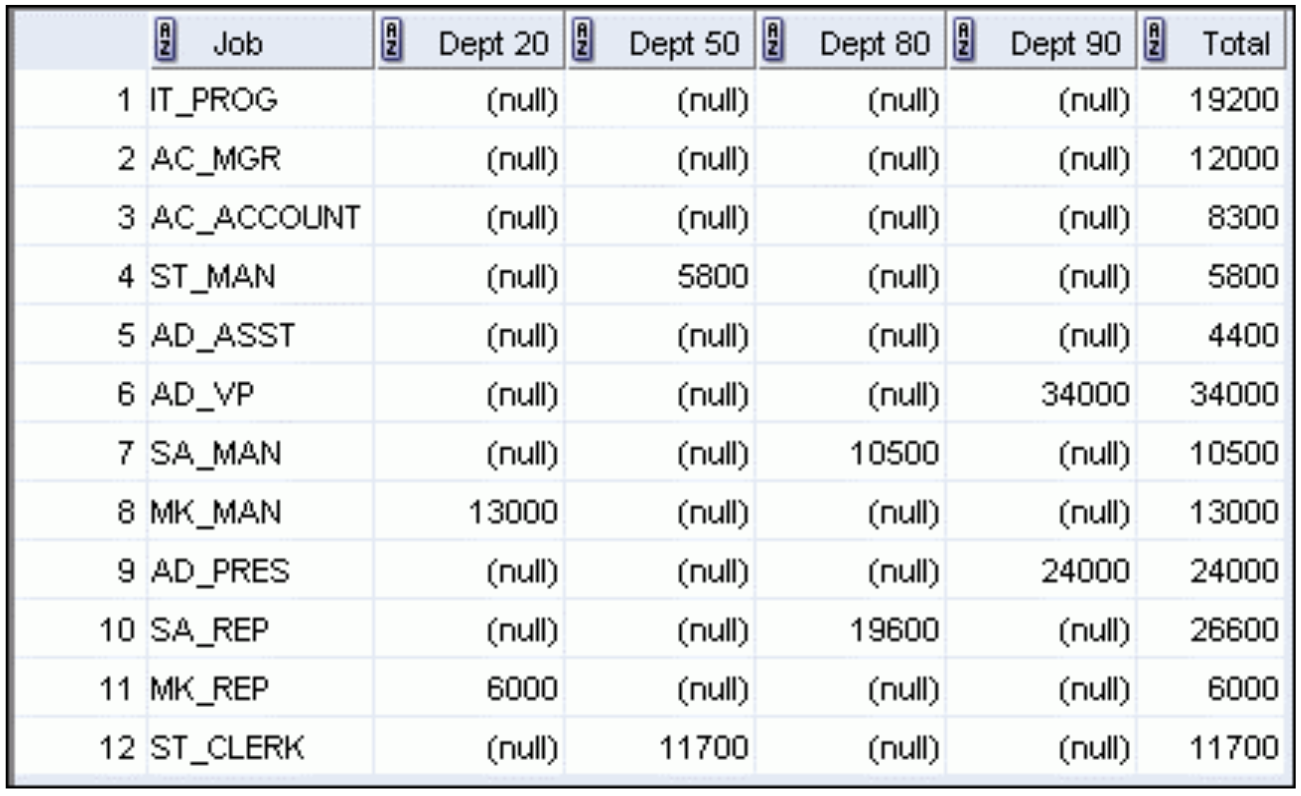
\includegraphics[width=.7\linewidth]{graphics/611.png}
    \end{figure}

    \textbf{Solution: }
    \begin{lstlisting}[language=SQL]
SELECT job_id AS "Job",
    SUM(CASE WHEN department_id = 20 
        THEN salary ELSE NULL END) AS "Dept 20",
    SUM(CASE WHEN department_id = 50 
        THEN salary ELSE NULL END) AS "Dept 50",
    SUM(CASE WHEN department_id = 80 
        THEN salary ELSE NULL END) AS "Dept 80",
    SUM(CASE WHEN department_id = 90 
        THEN salary ELSE NULL END) AS "Dept 90",
    SUM(salary) AS "Total"
FROM hr. employees
WHERE department_id IN (20, 50, 80, 90)
GROUP BY job_id
ORDER BY job_id;

    \end{lstlisting}
\end{enumerate}
\end{document}
